\section{Gold-PVD}
\label{goldpvd}

Als Testsystem für PVD-Prozesse bietet sich Gold-PVD an, mit der Goldschichten epitaktisch auf monokristallinen Substraten aufgewachsen werden können\cite{gottsche_uber_1956}, für amorphe oder polykristalline Substrate aber durch Bildung von Nanopartikeln polykristalline Schichten erzeugt werden\cite{svorcik_annealing_2011}.
Die Zielsetzung für die Untersuchungen der Gold-PVD bestehen in der Voruntersuchung des MD-Potentiales, der Simulation epitaktischer Abscheidungen auf dünnen und nanostrukturierten Gold-Substraten und der Simulation von Abscheidungen auf gröberen Strukturen.
Die genutzte EAM-Potentialparametrisierung wird mit dem LAMMPS-Paket\cite{plimpton_lammps_2014} verbreitet, basiert aber auf Parametern von \textsc{Foiles et al.}\cite{foiles_embedded-atom-method_1986}, die für die Einbettung einzelner Atome in Bulk- und Oberflächensysteme optimiert wurden und somit den Abscheidungsprozess auf atomistischer Ebene ideal darstellen sollten.

\subsection{Voruntersuchungen}
\label{goldpreparation}

Zur Validierung grundlegender Materialeigenschaften von kristallinem Gold wurden Bindungslängen, Dichten und Koordinationszahlen aus einer relaxierten kristallinen Phase untersucht und mit experimentellen Werten\cite{haynes_crc_2011} verglichen (Tabelle~\ref{tab:goldpreresults}).
Eine gesammelte Übersicht der experimentellen Werte ist in Anhang~\ref{appendix_constants} zu finden.
In der MD-Simulation wurde ein Goldkristall mit einer Größe von \SI{40x40x40}{\angstrom} auf \SI{1000}{\kelvin} aufgeheizt (Schmelzpunkt: \SI{1337}{\kelvin}), im kanonischen Ensemble relaxiert und anschließend langsam abgekühlt, wobei die Dichte und die radiale Verteilungsfunktion bestimmt wurde.
Aus der radialen Verteilungsfunktion wurde anschließend die Bindungslänge und die Koordination bestimmt.

Bei diesem Prozess bleibt die Kristallstruktur erhalten und steht in guter Übereinstimmung mit den Literaturwerten.
Somit unterstützt die genutzte EAM-Para\-metri\-sierung das Zielsystem hinsichtlich der Dichte und Struktur monokristalliner Bulkmaterialien.

\begin{table}[t]
  \begin{threeparttable}
  \oddrowcolors
  \caption[Vergleich der strukturellen Eigenschaften von Gold mit Literaturdaten]{
    Vergleich der strukturellen Eigenschaften von Gold mit Literaturdaten\cite{haynes_crc_2011}
  }
  \label{tab:goldpreresults}
  \begin{tabularx}{\textwidth}{|lXXXX|}
    \hline
    \textbf{unters. Größe} & \textbf{Temperatur} & \textbf{Simulation}                     & \textbf{Referenz}\tnote{a}              & \textbf{Abweichung} \\
    \hline
    Bindungslänge          & \SI{300}{\kelvin}   & \SI{2.885}{\angstrom}                   & \SI{2.884}{\angstrom}                   & \SI{0.05}{\percent} \\
    Koordination           & \SI{300}{\kelvin}   & \SI{12.00}{}                            & \SI{12.00}{}                            & \SI{0}{\percent}    \\
    Dichte                 & \SI{300}{\kelvin}   & \SI{18.99}{\gram\per\cubic\centi\meter} & \SI{19.30}{\gram\per\cubic\centi\meter} & \SI{-1.6}{\percent} \\
    Dichte                 & \SI{500}{\kelvin}   & \SI{18.89}{\gram\per\cubic\centi\meter} & \SI{19.13}{\gram\per\cubic\centi\meter} & \SI{-1.2}{\percent} \\
    \hline
  \end{tabularx}
  \begin{tablenotes}
    \item[a] Referenzwerte stammen aus Referenz\cite{haynes_crc_2011} oder sind daraus berechnet.
      Siehe Anhang~\ref{appendix_constants}
  \end{tablenotes}
  \end{threeparttable}
\end{table}

\subsection{Thermodynamische Eigenschaften}
\label{goldthermo}

\begin{figure}[b!]

  \centering
  \captionsetup[subfigure]{singlelinecheck=false}

  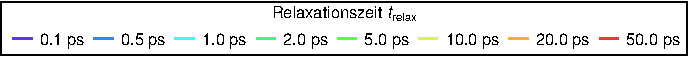
\includegraphics[width=0.97\textwidth]{gold_trelax_legend}

  \def\subfigwidth{7cm}
  \begin{subfigure}[t]{\subfigwidth}
    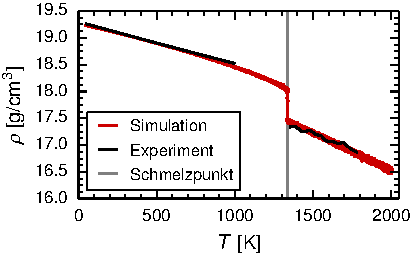
\includegraphics[width=\textwidth]{gold_bestthermo}
    \subcaption{Dichte bei $ t_\text{relax}=\SI{50}{\pico\second}$ und $\tau=\SI{0.02}{\femto\second}$}
    \label{fig:goldthermo-a}
  \end{subfigure}
  \hfill
  \begin{subfigure}[t]{\subfigwidth}
    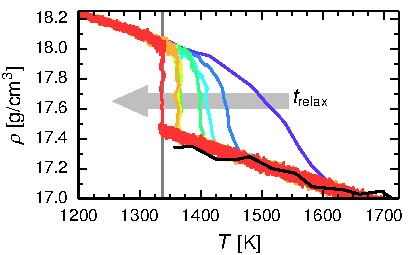
\includegraphics[width=\textwidth]{gold_trelax}
    \subcaption{Phasenübergang in Abh. von $t_\text{relax}$}
    \label{fig:goldthermo-b}
  \end{subfigure}

  \caption[Vergleich thermodynamischer Daten von Gold]{
    Vergleich thermodynamischer Daten von Gold für unterschiedliche Relaxationszeiten.
    Experimentelle Werte stammen aus Referenzen~\cite{haynes_crc_2011,brillo_density_2006}.
  }
  \label{fig:goldthermo}
\end{figure}

Neben strukturellen Eigenschaften bilden EAM-Potentiale auch einige thermodynamische Eigenschaften von Metallen ab, von denen aufgrund der potentiell hohen Substrattemperaturen bei PVD-Prozessen\cite{gottsche_uber_1956} anhand der Dichte der Phasenübergang an der Schmelztemperatur untersucht werden soll.
Dafür wurde in MD-Simulationen ein Gold-Kristall mit einer Größe von \SI{40x40x40}{\angstrom} schrittweise von \SI{50}{\kelvin} auf \SI{2000}{\kelvin} im isotherm-isobaren Ensemble erwärmt, wobei der Schmelzpunkt bei \SI{1337}{\kelvin}\cite{haynes_crc_2011} überschritten wurde.
Die Relaxationszeit $t_\text{relax}$ nach jedem Temperaturschritt von \SI{50}{\kelvin} und die Thermostat-Dämpfung $\tau$ wurden dabei variiert, um ihren Einfluss auf die Aussagekraft der Simulation zu untersuchen.

Die Ergebnisse zeigen gute Übereinstimmung mit experimentellen Daten\cite{haynes_crc_2011,brillo_density_2006} (Abbildung~\ref{fig:goldthermo}), wofür Relaxationszeiten $t_\text{relax} > \SI{20}{\pico\second}$ und Thermostat-Dämpfungsparameter $\tau = \SI{20}{\femto\second}$ bei einer Zeitschrittweite von $\Delta t = \SI{1}{\femto\second}$ für die Relaxation im isotherm-isobaren Ensemble als notwendig ermittelt wurden.
Bei geringeren $t_\text{relax}$ oder $\tau$ relaxiert das System innerhalb eines Temperaturschrittes nicht vollständig, wodurch der Schmelzpunkt überschätzt wird (Abbildung~\ref{fig:goldthermo-b}).
Darin zeigt sich auch eine Änderung in der Art des Phasenüberganges, der durch erhöhte Relaxationszeiten aufgrund von zeitlichen Effekten verzögert eintritt.
Das ergibt sich aus der Ähnlichkeit der Relaxationszeit zur Barostat-Dämpfung ($t_\text{relax}\approx \tau_p$), welche um Größenordnungen unter dem notwendigen Wert liegen (Abschnitt~\ref{mdmethods}), sodass sich das thermische Gleichgewicht nicht im Zeitrahmen der Simulation einstellen kann.

Somit lässt sich Gold mit der verwendeten EAM-Parametrisierung bei verschiedenen Temperaturen zuverlässig beschreiben, sofern die Relaxationszeit ausreichend groß eingestellt ist.
Für Parsivald-Rechnungen sind durch Nutzung der nur teilperiodischen Räume keine Barostate notwendig, wodurch die Relaxationszeit lediglich die kürzeren Perioden der Temperatur-Oszillationen, die vom Thermostat verursacht werden, abdecken muss.
In den nachfolgenden Simulationen mit EAM-Potentialen wird deshalb $t_\text{relax} = 5 \tau$ gewählt.

\subsection{Simulation von Gold-PVD}

In einer Parsivald-Simulation wurde auf einem kristallinen Substrat mit einer Oberfläche von \SI{106x106}{\angstrom} an der (001)-Kristallebene im PVD-Modus über 100 Parsivald-Zyklen ein Goldfilm abgeschieden.
Es wurden dafür MD-Boxen mit einer Größe von \SI{37x37x25}{\angstrom} mit jeweils ca. \num{1800} Atomen, Relaxationszeiten von \SI{1.4}{\pico\second} in \num{1400} Simulationsschritten und Auftreffgeschwindigkeiten von \SI{4}{\angstrom/\pico\second} genutzt.
Letztere liegen mit \SI{16.7}{\electronvolt} leicht oberhalb der üblichen Teilchenenergien von \SIrange{1}{10}{\electronvolt}\cite{thompson_ii._1968}, werden aber vor dem eigentlichen Auftreffen durch das Thermostat, welches unvermeidlich auch das auftreffende Atom betrifft, reduziert.
Zur Korrektur dieses systematischen Fehlers wäre eine Aufteilung des Zeit-Integrators der MD-Simulation in einen kanonischen und einen mikrokanonischen Teil notwendig, was mit einem erhöhten Rechenaufwand für jeden Zeitschritt verbunden ist.
Wie im vorherigen Abschnitt untersucht, hat die Temperatur in der MD-Simulation keinen Einfluss auf die grundlegende Struktur, weshalb eine leichte Überschätzung der Teilchenenergie und der damit einhergehenden Temperatur nach Auftreffen des Teilchens toleriert wird.
Ein mögliches Problem besteht hier in dem Herausschlagen von Teilchen aus der Oberfläche, allerdings sind die Energie dafür unterhalb typischer Sputter-Energien im Bereich mehrerer \SI{}{\kilo\electronvolt}\cite{mattox_handbook_2010}, mit denen Teilchen auf dem Target auftreffen und die in dieser Simulation betrachteten Atome heraus schlagen.

\begin{figure}[t]
  \captionsetup[subfigure]{singlelinecheck=false}
  \def\subfigwidth{0.49\textwidth}

  \begin{subfigure}[t]{\subfigwidth}
    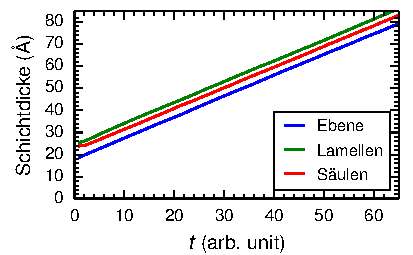
\includegraphics[width=\textwidth]{gold_thickness}
    \subcaption{Zeitverlauf der Schichtdicke}
    \label{fig:goldsmooth-a}
  \end{subfigure}
  \hfill
  \begin{subfigure}[t]{\subfigwidth}
    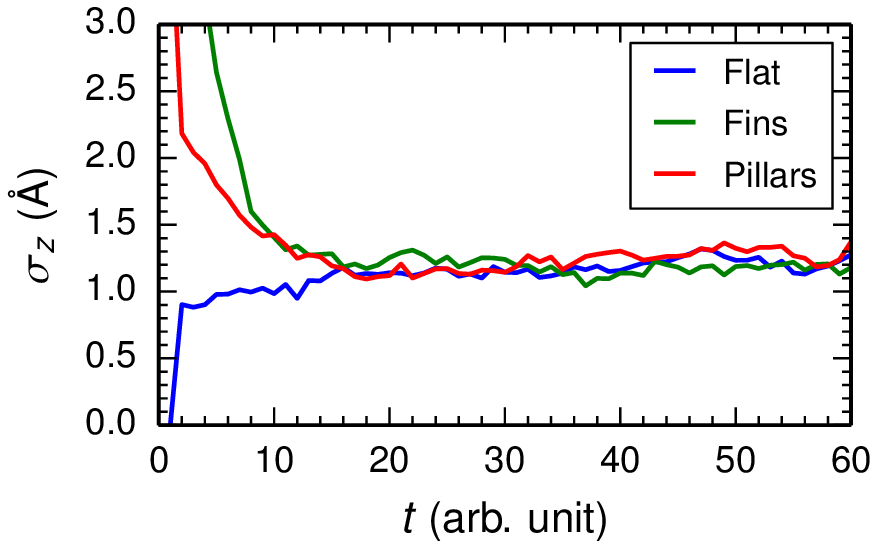
\includegraphics[width=\textwidth]{gold_goodroughness}
    \subcaption{Zeitverlauf der Rauheit}
    \label{fig:goldsmooth-b}
  \end{subfigure}

  \caption[Schichteigenschaften von Gold auf glatten Substraten]{
    Entwicklung der Schichteigenschaften von Gold auf glatten Substraten
  }
  \label{fig:goldsmooth}

\end{figure}

Die Simulationen zeigen epitaktisches Wachstum von Gold-Schichten (Abbildungen~\ref{fig:goldsmooth-a} und~\ref{fig:golddepositions-d}) mit einer RMS-Rauheit (Root Mean Square, Standardabweichung) von \SI{1.2}{\angstrom}, die somit unterhalb der Bindungslänge von \SI{2.884}{\angstrom} liegt und über den Simulationszeitraum konstant bleibt (Abbildung~\ref{fig:goldsmooth-b}).
Experimentelle Werte zur Rauheit von epitaktisch abgeschiedenen Gold-Filmen wurden nicht gefunden werden, doch liegen die simulierten Werte unterhalb der Rauheit von \SIrange{11}{18}{\nano\meter} für polykristalline Schichten, die per PVD auf Glas-Substraten abgeschieden wurden\cite{svorcik_annealing_2011}.
Diese sind allerdings durch die Bildung von Goldpartikel dominiert, wohingegen die simulierten Atome bereits auf perfekten monokristallinen Strukturen auftreffen.
Da Gold auch auf anderen Kristallstrukturen und ungeordneten Substraten eine Affinität zu kristallinem Wachstum zeigt\cite{gottsche_uber_1956,everitt_evolution_2000}, wirken die Ergebnisse der Parsivald-Simulation plausibel.
Eine Untersuchung amorpher und polykristalliner Substrate wäre für bessere Vergleichbarkeit mit Experimenten\cite{adamov_electrical_1974} interessant, übersteigt jedoch den Rahmen der Arbeit.
Poren und Hohlräume wurden bei Untersuchungen per Alpha-Form (Abschnitt~\ref{mdmethods-surface}) nicht gefunden, sodass die Gold-Atome in einem perfekten fcc-Gitter arrangiert sind.

Ergänzend wurde zur Prüfung der Robustheit des Parsivald-Prozesses nanostrukturierte Substrate in Form von \SI{1}{\nano\meter} breiten Lamellen und Säulen vorbereitet, auf welchen sich nach kurzer Simulationszeit glatte Schichten gebildet haben, die keine Unterschiede zu den Schichten auf dem glatten Substrat zeigen.

\subsubsection{Simulation von Abscheidungen auf strukturierten Substraten}

Neben der Abscheidung auf glatten Substraten wurden am Beispiel der Gold-PVD auch Abscheidungen auf strukturierten Substraten mit identischen Prozessbedingungen simuliert (Abbildung~\ref{fig:golddepositions}).
Dafür wurden Substrate präpariert, welche die Form von Schwellen oder Spitzen mit einer Höhe von \SI{20}{\angstrom}, einer Breite von \SI{50}{\angstrom} und Neigungen von \SI{15}{\degree}, \SI{20}{\degree}, \SI{30}{\degree}, \SI{45}{\degree}, \SI{60}{\degree} und \SI{90}{\degree} annehmen (Abbildungen~\ref{fig:golddepositions-b} und~\ref{fig:golddepositions-c}).
Auf vorherige Relaxierung der Substrate wurde aufgrund der Stabilität sowie der relaxierenden Eigenschaften der MD-Ereignisse verzichtet.
Dadurch können sich an den Wänden der Schwellen und Spitzen auch ungünstige Schnitte durch die Einheitszellen ergeben, die in den weiteren Untersuchungen aber nicht maßgeblich für die Struktur der abgeschiedenen Schichten sind.

\begin{figure}[t]
  \captionsetup[subfigure]{singlelinecheck=false}
  \def\subfigwidth{0.49\textwidth}

  \begin{subfigure}[t]{\subfigwidth}
    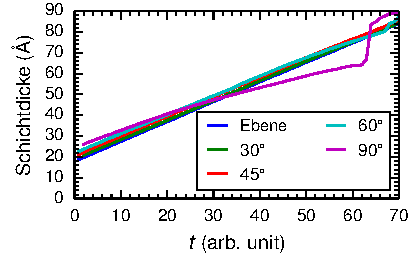
\includegraphics[width=\textwidth]{goldtipthickness}
    \subcaption{Zeitverlauf der Schichtdicke}
    \label{fig:goldrough-a}
  \end{subfigure}
  \hfill
  \begin{subfigure}[t]{\subfigwidth}
    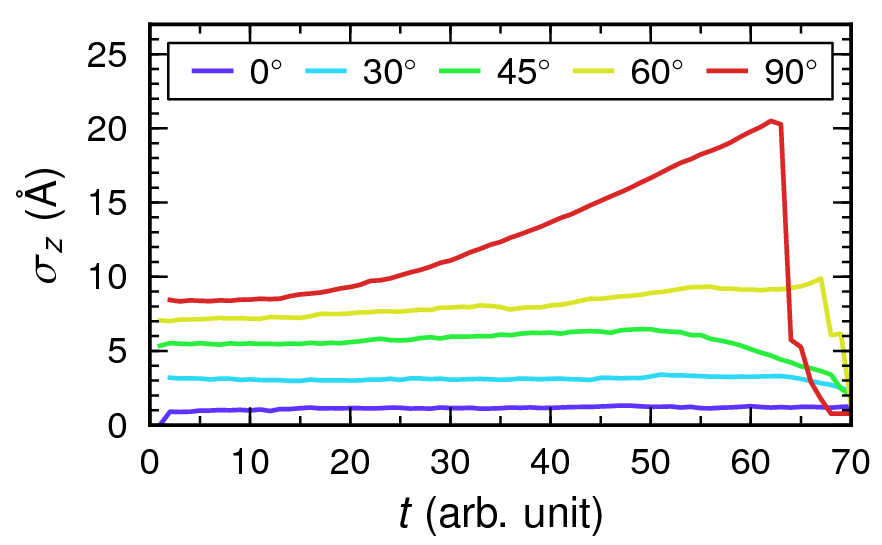
\includegraphics[width=\textwidth]{gold_tiproughness_s70}
    \subcaption{Zeitverlauf der Rauheit}
    \label{fig:goldrough-b}
  \end{subfigure}

  \caption[Schichteigenschaften von Gold auf strukturierten Substraten]{
    Entwicklung der Schichteigenschaften von Gold auf strukturierten Substraten
  }
  \label{fig:goldrough}

\end{figure}

\begin{figure}[p]
  \captionsetup[subfigure]{singlelinecheck=false}
  \def\subfigwidth{0.31\textwidth}
  \begin{subfigure}[t]{\subfigwidth}
    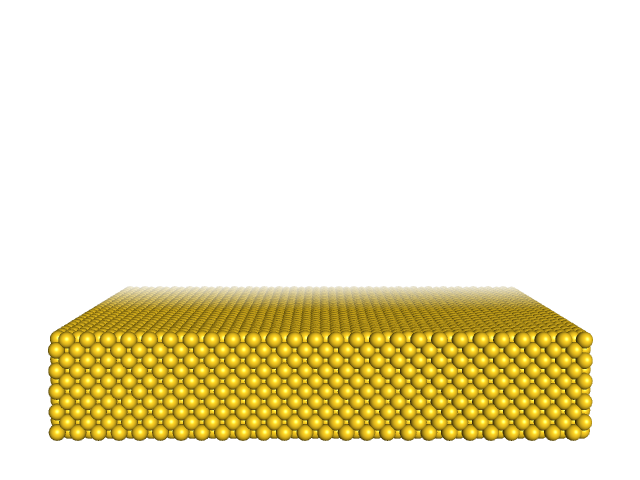
\includegraphics[width=\textwidth]{Au_substrate_flat}
    \subcaption{Glattes Gold-Substrat}
    \label{fig:golddepositions-a}
  \end{subfigure}
  \hfill
  \begin{subfigure}[t]{\subfigwidth}
    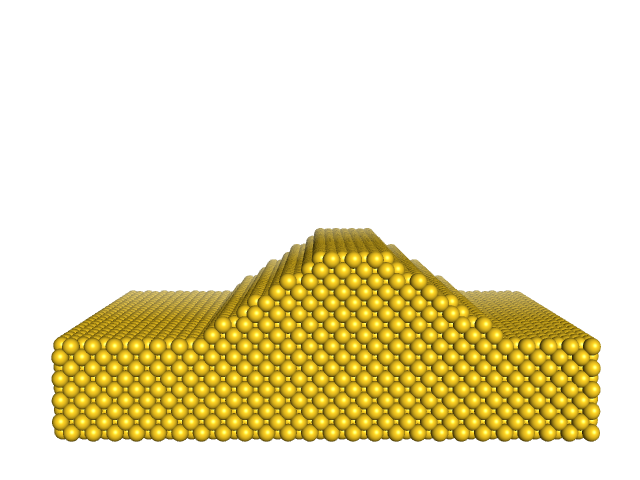
\includegraphics[width=\textwidth]{Au_substrate_step30}
    \subcaption{Gold-Schwelle, \SI{30}{\degree}}
    \label{fig:golddepositions-b}
  \end{subfigure}
  \hfill
  \begin{subfigure}[t]{\subfigwidth}
    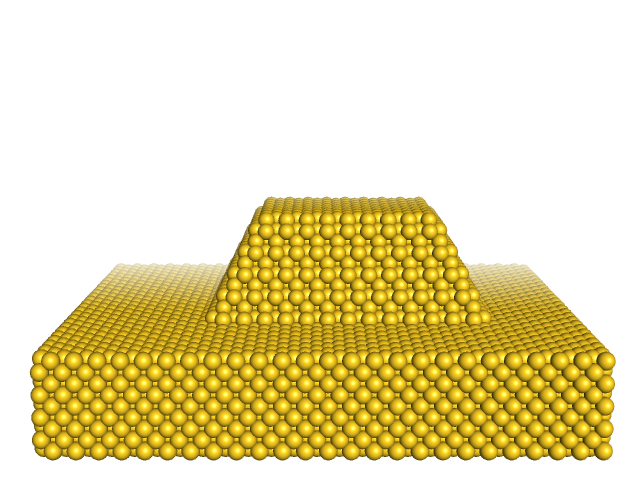
\includegraphics[width=\textwidth]{Au_substrate_tip60}
    \subcaption{Gold-Spitze, \SI{60}{\degree}}
    \label{fig:golddepositions-c}
  \end{subfigure}

  \LARGE\center{$\Downarrow$}
  \vspace{0.25cm}

  \captionsetup[subfigure]{singlelinecheck=false}
  \def\subfigwidth{0.31\textwidth}
  \begin{subfigure}[t]{\subfigwidth}
    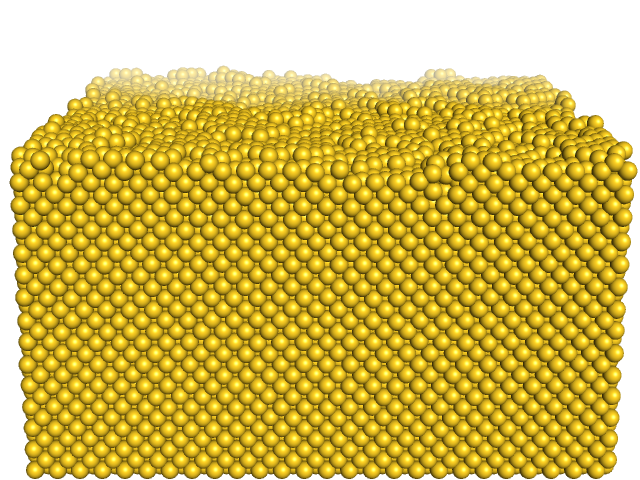
\includegraphics[width=\textwidth]{Au_deposition_flat}
    \subcaption{Glatte, kristalline Schicht ($\sigma_z = \SI{1.2}{\angstrom}$)}
    \label{fig:golddepositions-d}
  \end{subfigure}
  \hfill
  \begin{subfigure}[t]{\subfigwidth}
    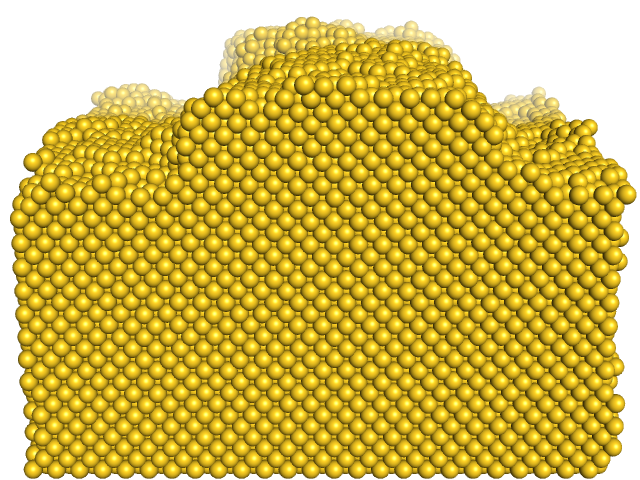
\includegraphics[width=\textwidth]{Au_deposition_step30}
    \subcaption{Fortsetzung der Schwelle ($\sigma_z = \SI{6.4}{\angstrom}$)}
    \label{fig:golddepositions-e}
  \end{subfigure}
  \hfill
  \begin{subfigure}[t]{\subfigwidth}
    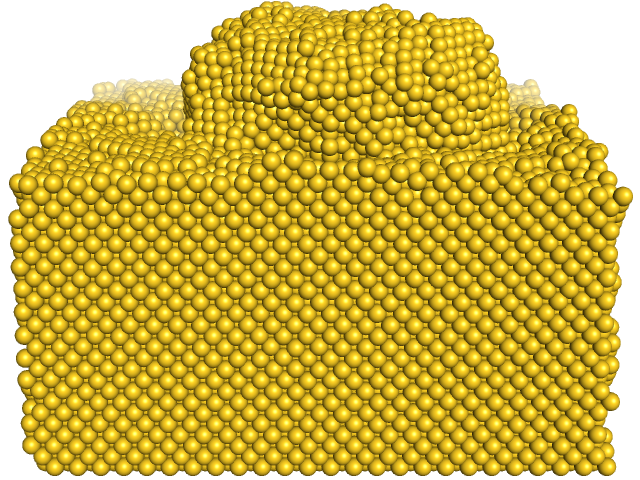
\includegraphics[width=\textwidth]{Au_deposition_tip60}
    \subcaption{Fortsetzung der Spitze ($\sigma_z = \SI{8.0}{\angstrom}$)}
    \label{fig:golddepositions-f}
  \end{subfigure}
  \caption[Gold-PVD auf strukturierten Substraten]{
    Goldschicht nach \num{50} Abscheidungsschritten (\SI{47}{\angstrom}) auf strukturierten Substraten
  }
  \label{fig:golddepositions}
\end{figure}

\begin{figure}[p]
  \captionsetup[subfigure]{singlelinecheck=false}
  \def\subfigwidth{0.49\textwidth}

  \begin{subfigure}[t]{\subfigwidth}
    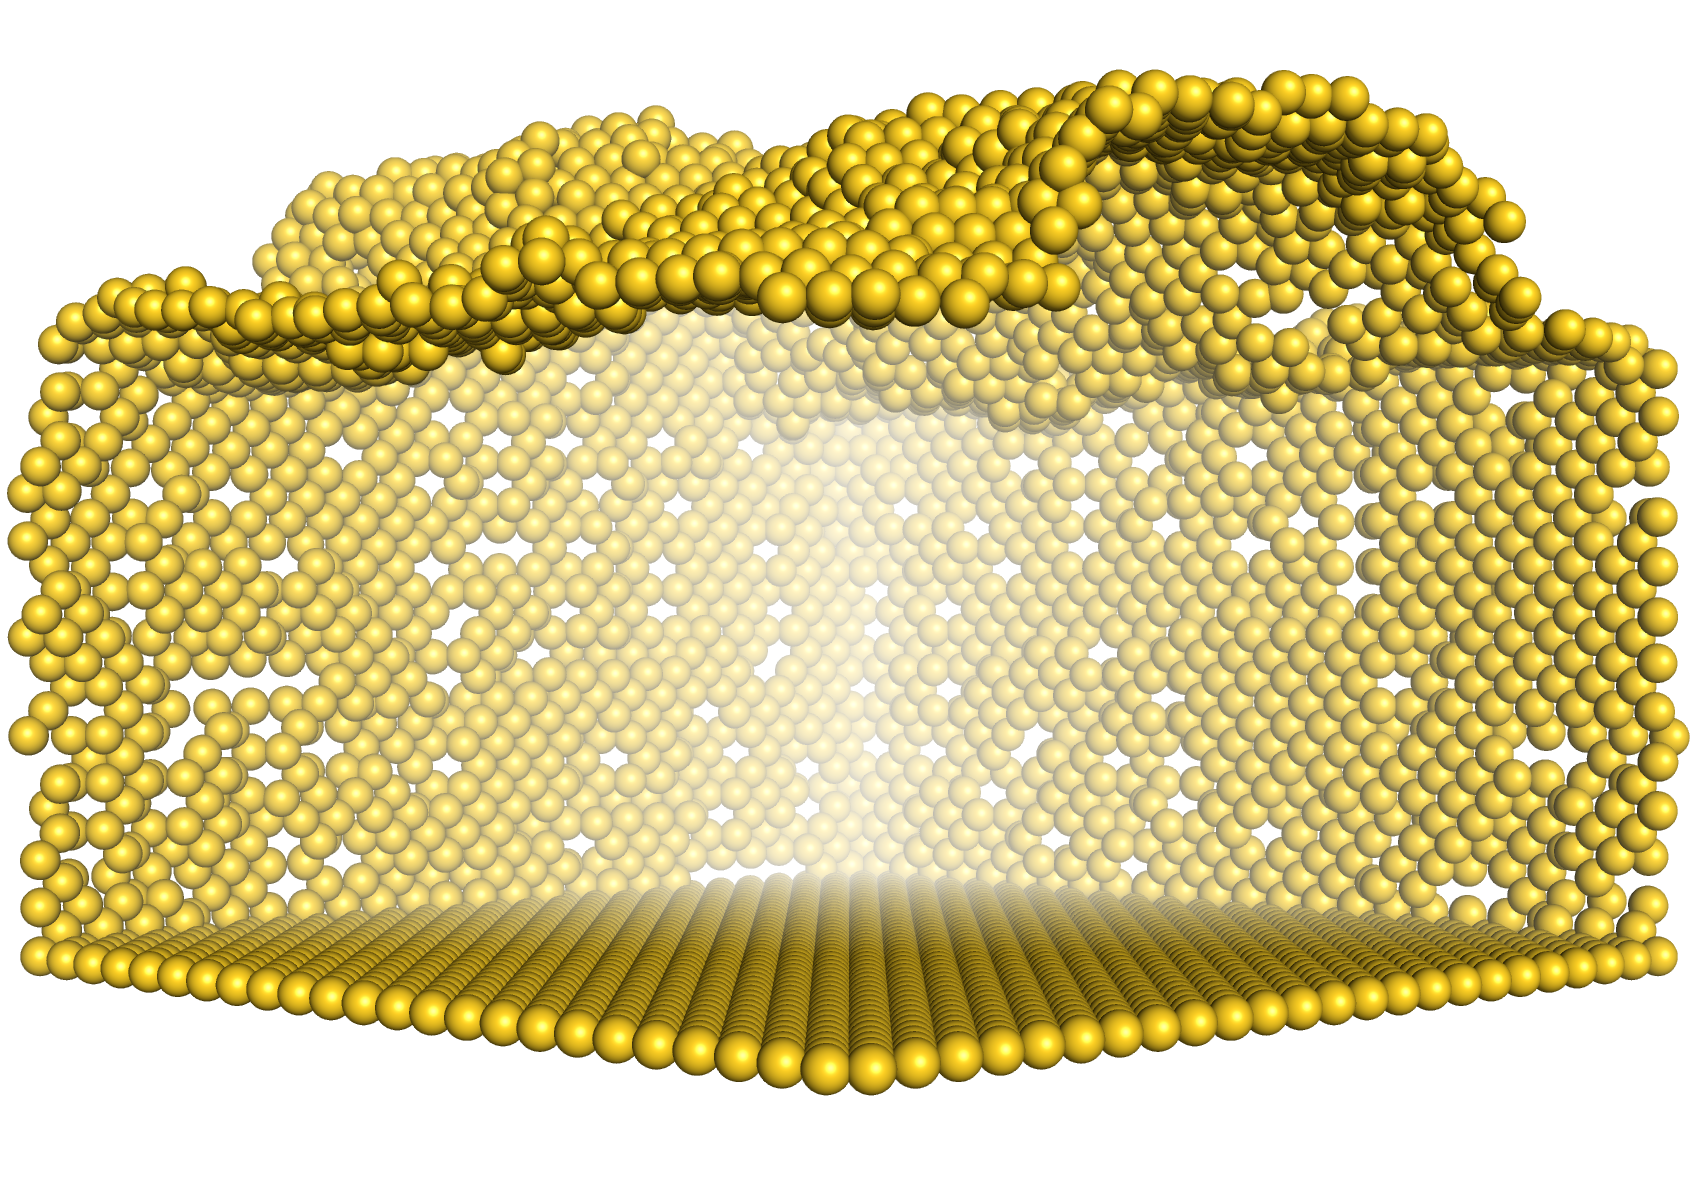
\includegraphics[width=\textwidth]{gold_step30_pockets}
    \subcaption{Alpha-Form der \SI{30}{\degree}-Schwelle}
    \label{fig:goldpockets-a}
  \end{subfigure}
  \hfill
  \begin{subfigure}[t]{\subfigwidth}
    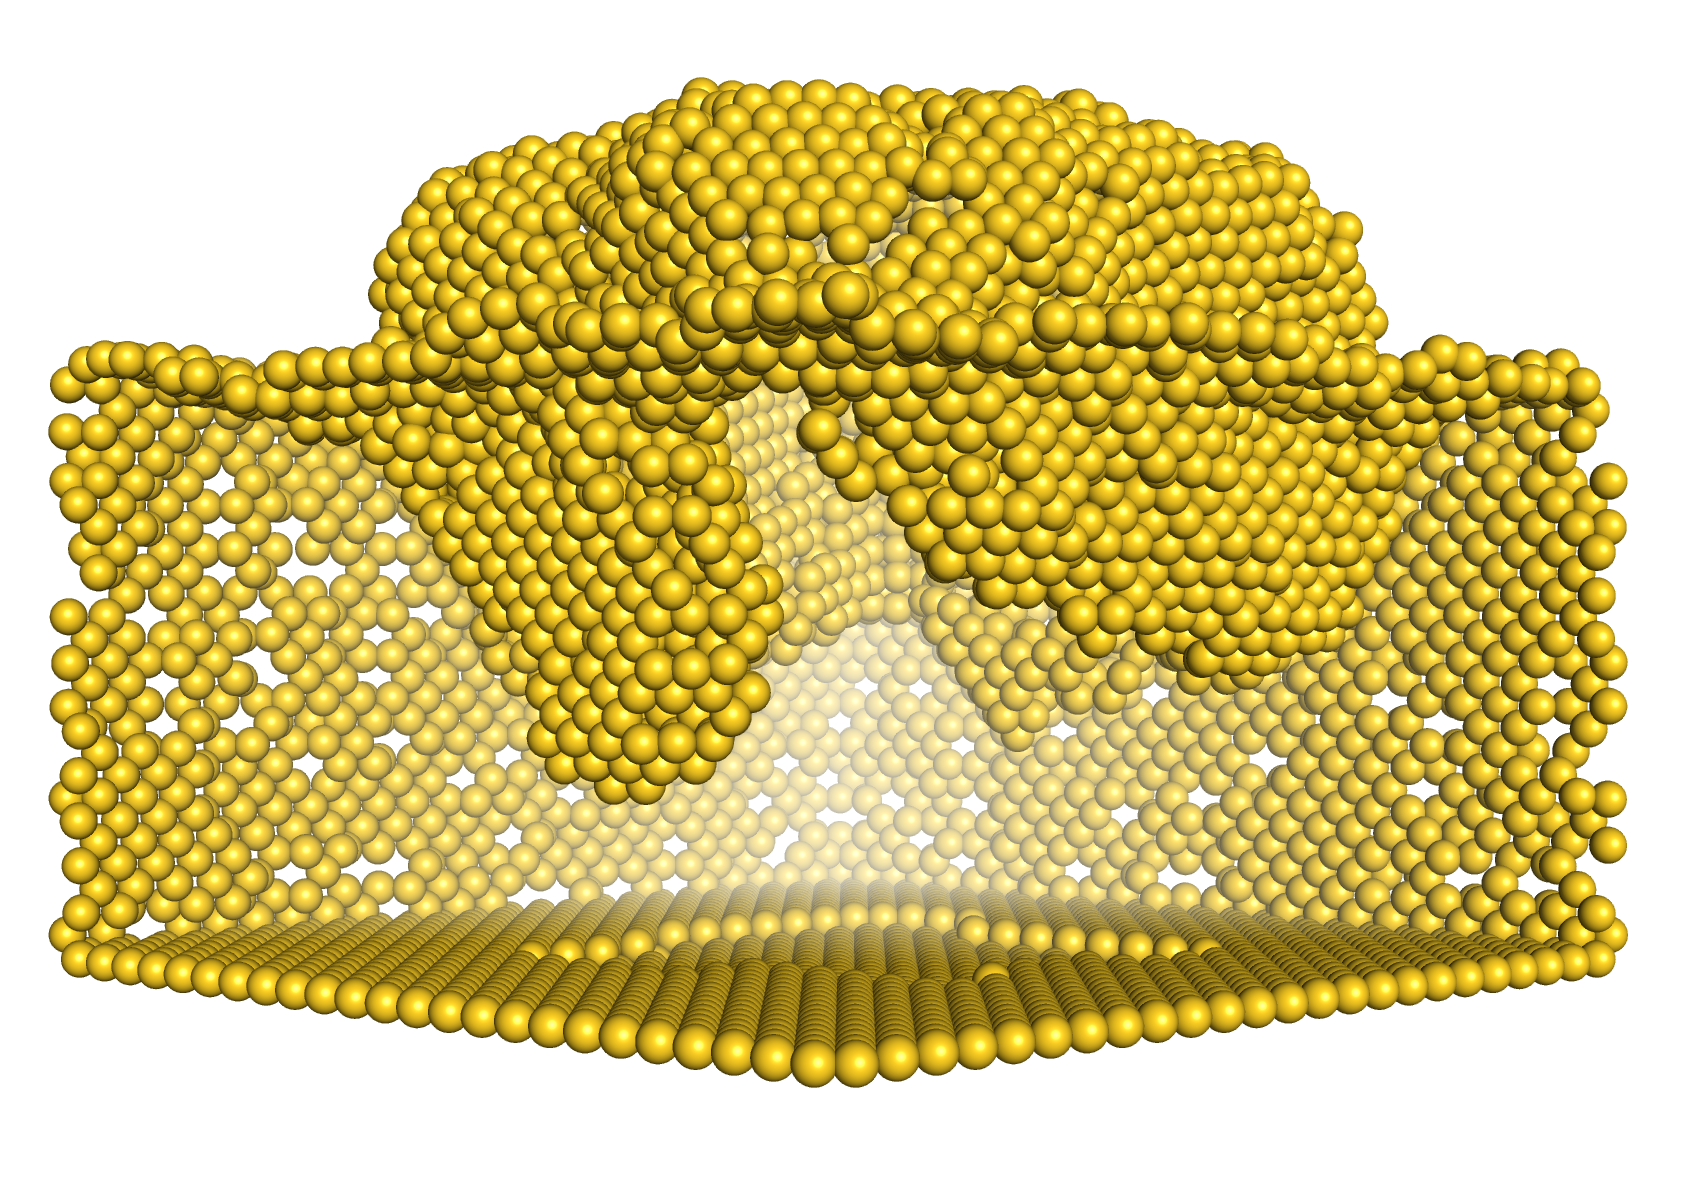
\includegraphics[width=\textwidth]{gold_tip90_pockets}
    \subcaption{Alpha-Form der \SI{90}{\degree}-Spitze}
    \label{fig:goldpockets-b}
  \end{subfigure}

  \caption[Porenbildung bei Gold-Strukturen]{Porenbildung bei Gold-Strukturen über \num{40} Schritte (\num{22000} Ereignisse $\hat{=}$ \SI{38}{\angstrom}).
  }
  \label{fig:goldpockets}
\end{figure}

Die Schichtdicken aus den Abscheidungssimulationen auf strukturierten Substraten unterscheiden sich nicht signifikant von den für glatte Substrate gewonnenen Werten, mit Ausnahme der \SI{90}{\degree}-Strukturen.
Die abgeschiedenen Schichten wachsen ebenfalls epitaktisch auf, bilden aber Hohlräume und Nanoporen, wodurch sich kein perfekter Kristall ergibt.
In der Rauheit bestehen Unterschiede zur Simulation von Abscheidungen auf glatten Substraten (\SI{0}{\degree}) in einer generell erhöhten Rauheit, die für geringe Neigungswinkel allerdings konstant bleibt.

Für extreme Neigungswinkel von \SI{90}{\degree} ist eine Zunahme der Rauheit zu beobachten, welche durch die Bildung von Nanoporen an der Basis der Spitzen und Schwellen in der Simulation verursacht wird (Abbildung~\ref{fig:goldpockets}).
Dabei handelt es sich um ein Artefakt der Oberflächensuche der Parsivald-Simulation, die von oben eine senkrechte Suche nach dem höchsten Punkt in der xy-Ebene durchführt.
Somit werden an geneigten Flächen höher gelegene Abscheidungsorte mit größeren Neigungen bevorzugt, wobei oberhalb von \SI{90}{\degree} von einer vollständigen Abschirmung eines Teils der Oberfläche auszugehen ist.
Dadurch bilden sich Nanoporen an der Basis von Spitzen und Schwellen, die sich im weiteren Verlauf der Simulationen verengen, bis sie schließlich zu Hohlräumen abgeschlossen werden.
In der Auswertung macht sich der Abschluss durch einen rapiden Abfall der Rauheit bemerkbar, die sich aus der Eigenschaft der Alpha-Form ergibt, die gesamte Nanopore als Teil der Oberfläche anzusehen, sodass nach ihrer Schließung die mittlere Höhe der Oberfläche schlagartig zunimmt.

\subsection{Skalierbarkeit mit der Simulationsgröße}
\label{goldscalability}

\begin{table}[t]
  \begin{threeparttable}

    \caption[Laufzeitgrößen von Parsivald für Gold-PVD]{
      Laufzeitgrößen von Parsivald für Gold-PVD bei unterschiedlichen $w_\text{sim}$
    }
    \label{tab:goldscalability}

    \begin{tabularx}{\textwidth}{|Xrrrrrrr|}
      \hline
      \textbf{$w_\text{sim}$} & \textbf{Wachst.}    & \textbf{Atome} & \textbf{$N_\text{E}$} & \textbf{Worker\tnote{a} $p$}          & \textbf{$\rho_\text{work.}$} & \textbf{$T_\text{p}$} & \textbf{RAM}\tnote{b} \\
      \hline
      \SI{106}{\angstrom}     & \SI{70}{\angstrom}  & \num{59549}    & \num{46030}           & \num{1.8}\tnote{c}        (\num{4})   & \SI{21.9}{\percent}          & \SI{32.2}{\hour}      & \SI{254}{\mebi\byte}  \\
%%    \SI{204}{\angstrom}     & \SI{42}{\angstrom}  & \num{152374}   & \num{102374}          & \num{14.5}\tnote{c}       (\num{18})  & \SI{13.9}{\percent}          & \SI{25.5}{\hour}      & \SI{257}{\mebi\byte}  \\
      \SI{204}{\angstrom}     & \SI{94}{\angstrom}  & \num{278702}   & \num{228702}          & \num{5.33}\tnote{c}       (\num{12})  & \SI{17.5}{\percent}          & \SI{55.1}{\hour}      & \SI{259}{\mebi\byte}  \\
      \SI{500}{\angstrom}     & \SI{93}{\angstrom}  & \num{1708600}  & \num{1401081}         & \num{24.8}\tnote{c}       (\num{50})  & \SI{13.6}{\percent}          & \SI{73.6}{\hour}      & \SI{397}{\mebi\byte}  \\ % \SI{282}{\mebi\byte}
%%      \SI{1000}{\angstrom}  & \SI{5.4}{\angstrom} & \num{1591908}  & \num{381588}          & \num{44.8}                (\num{46})  & \SI{6.1}{\percent}           & \SI{1.5}{\hour}       & \SI{368}{\mebi\byte}  \\
      \SI{1000}{\angstrom}    & \SI{92}{\angstrom}  & \num{6733948}  & \num{5539942}         & \num{75.4}\tnote{c}       (\num{149}) & \SI{10.3}{\percent}          & \SI{97.5}{\hour}      & ~                     \\
      \SI{1}{\micro\meter}    & \SI{1.3}{\angstrom} & \num{1.3e8}    & \num{8186990}         & \num{25.4}\tnote{d}       (\num{46})  & \SI{0.03}{\percent}          & \SI{117.5}{\hour}     & \SI{11.5}{\gibi\byte} \\
%%    \SI{2}{\micro\meter}    & \SI{0.4}{\angstrom} & \num{4.9e8}    & \num{10356031}        & \num{26.3}\tnote{d}       (\num{46})  & \SI{0.009}{\percent}         & \SI{117.5}{\hour}     & ~                     \\
      \SI{2}{\micro\meter}    & \SI{1.0}{\angstrom} & \num{5.1e8}    & \num{25855695}        & \num{189}\tnote{e}        (\num{245}) & \SI{0.06}{\percent}          & \SI{186.8}{\hour}     & \SI{45.4}{\gibi\byte} \\
      \SI{4}{\micro\meter}    & ~                   & \num{1.9e9}    & ~                     & ~                         ~           & ~                            & ~                     & \SI{182}{\gibi\byte}  \\
      \hline
    \end{tabularx}

    \begin{tablenotes}
    \item[a] Mittelwert $p$ und beobachtetes Maximum der Zahl paralleler Worker
    \item[b] Vom Hostprozess verbrauchter Arbeitsspeicher.
    \item[c] $p = p_\text{max,1}$: Maximale Workerdichte erreicht
    \item[d] Inzwischen behobener Fehler in Parsivald hat Workerneustart verhindert
    \item[e] $p = p_\text{max,2}$: Ereignis-Durchsatz des Hostprozesses erreicht
    \end{tablenotes}

  \end{threeparttable}
\end{table}

Ein Vergleich mit den in Abschnitt~\ref{runtime} vorgestellten Laufzeitwerten wird im Folgenden anhand von Gold-PVD durchgeführt, für welche Abscheidungen auf unterschiedlich großen quadratischen Substraten mit Parsivald simuliert wurde.
Die Rechnungen wurden auf dem \textit{enssim}-Cluster des Fraunhofer ENAS und des Zentrums für Mikrotechnologien an der TU Chemnitz durchgeführt, bei welchem es sich um ein heterogenes System mit \num{912} Opteron- und \num{60} Xeon-Kernen handelt.
Sofern nicht anders angegeben, wurden die Hauptprozesse auf den schnellen Xeon-Kerne ausgeführt und ihnen ausreichend viele Worker zur Verfügung gestellt ($p > p_\text{max}$).

Aus Messungen ergeben sich die elementaren Laufzeiten als $T_\text{E} = \SI{26}{\milli\second}$ und $T_\text{MD} = \SI{4.7}{\second}$, während $w_\text{MD} = \SI{37}{\angstrom}$ fest gewählt und $w_\text{sim}$ von \SI{106}{\angstrom} bis \SI{4}{\micro\meter} variiert wurde, wobei auch der für die Beschichtung von Nanoelektronik interessante Bereich von \SIrange{100}{1000}{\nano\meter} untersucht wurde.
Dabei wurde, durch verschiedene Störeinflüsse bedingt, eine unterschiedliche Anzahl an Parsivald-Zyklen durchlaufen, sodass die Laufzeiten keinen direkten Vergleich zulassen.

Die Ergebnisse der Untersuchungen der Laufzeitgrößen sind in Tabelle~\ref{tab:goldscalability} zusammengefasst und stimmen gut mit den in Abschnitt~\ref{runtimeanalysis} ermittelten analytischen Werten überein (Abbildung~\ref{fig:goldscala}).
Die Zahl der möglichen Prozesse (Abbildung~\ref{fig:goldscala-workers}) steht für $\rho_\text{worker}=\SI{20}{\percent}$ in guter Übereinstimmung mit $p_\text{max}$, wobei die maximale effiziente Substratbreite als $w_\text{eff} \approx \SI{100}{\nano\meter}$ ermittelt wurde.
Für die mit $p_\text{max}$ verwandten Workerdichten $\rho_\text{worker}$ ist eine leichte Abnahme von \SI{21.9}{\percent} für $w_\text{sim} = \SI{106}{\angstrom}$ zu \SI{10.3}{\percent} für $w_\text{sim} = \SI{1000}{\angstrom}$ erkennbar, die danach jedoch quadratisch mit der Substratbreite abnimmt.
Es existiert ein Ausreißer bei $w_\text{sim} = \SI{1}{\micro\meter}$, für den nur 46 Worker gestartet wurden ($\num{46} < p_\text{max} \approx \num{190}$), die zudem durch einen inzwischen behobenen Fehler im Host-Worker-Code auf einen Wert von \num{25.4} unterschätzt wurden.

Ein Vergleich der Laufzeiten mit Werten für $T_p$ aus Gleichung~\ref{eq:runtime} zeigt ebenfalls gute Übereinstimmungen, wobei erneut der Ausreißer bei $w_\text{sim} = \SI{1}{\micro\meter}$ erkennbar ist (Abbildung~\ref{fig:goldscala-runtime}). %legitequationreference
Aufgrund der unterschiedlichen Auslastung der Rechenknoten durch Drittprozesse, der damit verbundenen variablen MD-Laufzeiten und der unterschiedlichen Schichtdicke lässt sich keine ideale Kurve in das Laufzeit-Diagramm eintragen, sodass nur einzelne Werte mit ihrer Vorhersage aus dem Modell (Abschnitt~\ref{runtime}) verglichen wurden.
Die Übereinstimmung mit den Modell-Werten bestätigt jedoch die gute Skalierbarkeit von Parsivald mit der Substratbreite.

Zuletzt zeigt die Auswertung der vom Hostprozess verbrauchten Ressourcen einen Speicherverbrauch von $\text{RAM} = \SI{253}{\mebi\byte} + \SI{94}{\byte} \cdot N_\text{Atome}$, womit auch große Simulationen mit \num{1.9e9} Atomen mit nur \SI{186}{\gibi\byte} Arbeitsspeicher durchgeführt werden können (Abbildung~\ref{fig:goldscala-memory}).
Somit stellt der verfügbare Arbeitsspeicher aktuell nur ein untergeordnetes Kriterium dar, jedoch spiegelt sich diese Größe auch in den von Parsivald geschriebenen atomistischen Dateien wider.
Mit bis zu \SI{75}{\gibi\byte} können diese nicht mehr effizient ausgewertet werden, wodurch eine Auswertung zur Zeit der Simulation unter Nutzung der effizienten Datenstrukturen notwendig wäre.

Somit bestätigen sich einige Vorhersagen aus Abschnitt~\ref{runtime}, jedoch sind weitere systematische Untersuchungen, etwa hinsichtlich der Ereignis-Laufzeit $T_\text{E}$, für einen umfassenden Vergleich notwendig.

\begin{figure}[t]
  \centering
  \captionsetup[subfigure]{singlelinecheck=false}
  \def\subfigwidth{7cm}
  \begin{subfigure}[t]{\subfigwidth}
    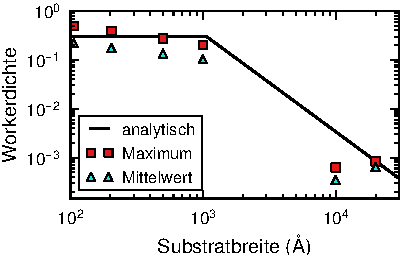
\includegraphics[width=\textwidth]{workerdichte}
    \subcaption{Workerdichte auf der Oberfläche (1=ideal)}
    \label{fig:goldscala-density}
  \end{subfigure}
  \hfill
  \begin{subfigure}[t]{\subfigwidth}
    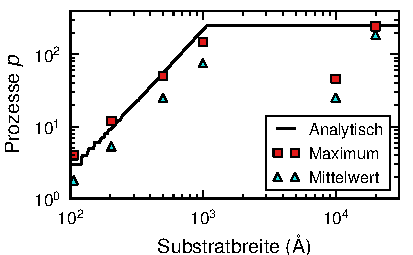
\includegraphics[width=\textwidth]{workers}
    \subcaption{Zahl der Parallelen Prozesse}
    \label{fig:goldscala-workers}
  \end{subfigure}

  \vspace{1em}

  \begin{subfigure}[t]{\subfigwidth}
    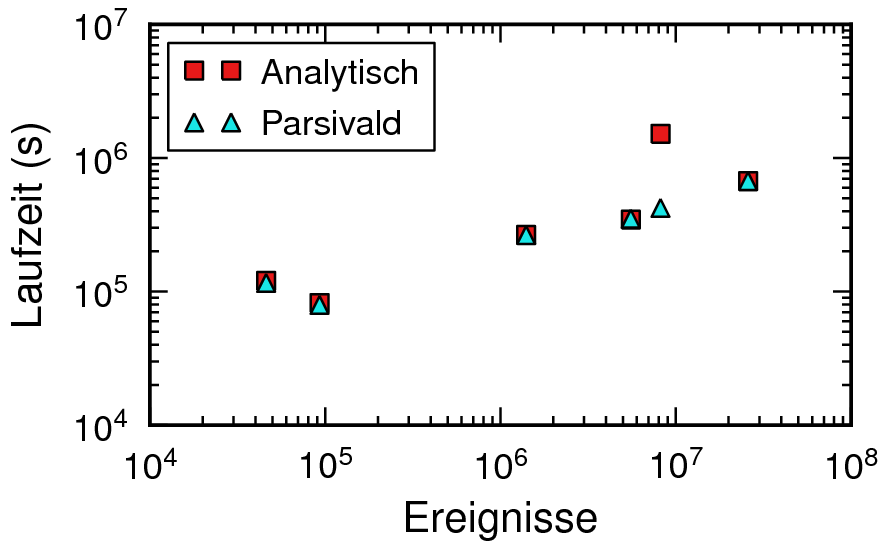
\includegraphics[width=\textwidth]{runtime}
    \subcaption{Laufzeit verschiedener Simulationen}
    \label{fig:goldscala-runtime}
  \end{subfigure}
  \hfill
  \begin{subfigure}[t]{\subfigwidth}
    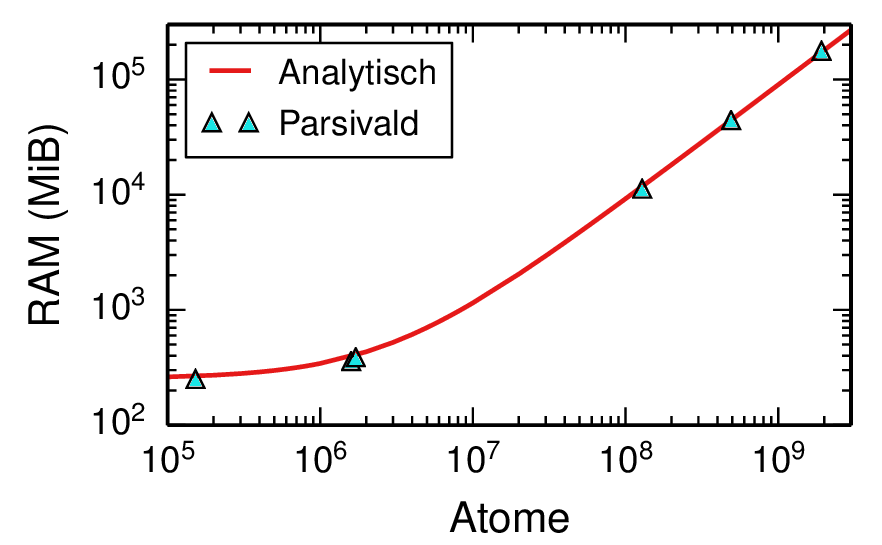
\includegraphics[width=\textwidth]{memory}
    \subcaption{Speicherverbrauch der Hauptprozesse}
    \label{fig:goldscala-memory}
  \end{subfigure}
  \caption[Vergleich der Parallelisierbarkeit zwischen dem Modell und PVD-Simulationen]{Parallelisierungseigenschaften von Parsivald im Vergleich zu dem Modell der Laufzeiteigenschaften (Abschnitt~\ref{runtime})}
  \label{fig:goldscala}
\end{figure}

\subsection{Fazit}

Mit Parsivald lässt sich Gold-PVD auf glatten und leicht strukturierten Substraten effizient simulieren, wobei sich durch epitaktisches Wachstum defektfreie kristalline Schichten auf glatten Substraten bilden.
Strukturierte Substrate sorgen in Parsivald-Simulationen hingegen für die Bildung von Nanoporen und Hohlräumen, die durch die aktuelle Implementierung des Parsivald-Modelles verursacht werden.
Eine mögliche Lösung wäre die implizite Betrachtung der Oberfläche mit Delaunay-Triangulationen, wie sie bereits für die Bestimmung der Alpha-Formen genutzt werden.
Damit würden auch schiefe Auftreffwinkel sowie eine bessere Betrachtung von CVD-Prozessen ermöglicht, die dafür bekannt sind, auch auf strukturierten Oberflächen konforme Schichten abzuscheiden\cite{granneman_thin_1993}.
